\chapter{Double Integrals and Application using Fubini's Theorem}
\label{chap:double-integrals-and-application-using-fubini-s-theorem}

\section{Review of the Definite Integrals}
\label{sec:review-of-the-definite-integrals}

\begin{equation}\label{eq:definite-integral}
  \int_{a}^{b}f(x)\,dx  
\end{equation}

\begin{definition}[Definite Integral as Area]
  \label{def:definite-integral}
  The definite integral of a function \(f(x)\) over the interval \([a,b]\) represents the net area under the curve from \(x = a\) to \(x = b\).
\end{definition}

\begin{remark}[Geometric Interpretation]
  If \(f(x) \geq 0\) on \([a,b]\), then the definite integral represents the area under the curve.
\end{remark}

\section{Double Integrals}
\label{sec:double-integrals}

\subsection{Double Integrals as Area, Volume and Average}
\label{ssec:double-integrals-as-area-volume-and-average}

\begin{definition}[Double Integral over Region]
  \label{def:double-integral}
  The double integral of \(f(x,y)\) over region \(R\) is denoted by:
  \begin{equation}\label{eq:double-integral}
    \iint_{R} f(x,y)\,dA
  \end{equation}
  where \(dA = dx\,dy\) or \(dA = dy\,dx\) depending on the order of integration.
\end{definition}

\begin{remark}[Area from Double Integral]
  When \(f(x,y) = 1\), the double integral \(\iint_R 1\,dA\) gives the area of region \(R\).
\end{remark}

\begin{explanation}[Volume Under Surface]
  If \(f(x,y) \geq 0\), then \(\iint_R f(x,y)\,dA\) represents the volume under the surface \(z = f(x,y)\) over region \(R\).
\end{explanation}

\begin{definition}[Average Value Over Region]
  \label{def:average-value}
  The average value of a function \(f(x,y)\) over a region \(R\) is given by:
  \begin{equation}\label{eq:average-value}
    \bar{f} = \frac{1}{\text{Area}(R)} \iint_R f(x,y)\,dA
  \end{equation}
\end{definition}

\begin{eg}[Average of \(f(x,y) = x + y\) over Unit Square]
  Let \(f(x,y) = x + y\), over the region \(R = [0,1] \times [0,1]\).

  \begin{align*}
    \iint_R f(x,y)\,dA &= \int_0^1 \int_0^1 (x + y)\,dx\,dy \\
                       &= \int_0^1 \left[ \int_0^1 x\,dx + \int_0^1 y\,dx \right] dy \\
                       &= \int_0^1 \left[ \frac{1}{2} + y \right] dy \\
                       &= \left[ \frac{1}{2}y + \frac{1}{2}y^2 \right]_0^1 \\
                       &= \frac{1}{2} + \frac{1}{2} = 1
  \end{align*}
\end{eg}

\section{Fubini's Theorem}
\label{sec:fubini-s-theorem}

\subsection{In Rectangular Region}
\label{ssec:in-rectangular-region}

\begin{theorem}
  For a rectangular region \(R: a \le x \le b\) and \(c \le y \le d\),
  \begin{equation}\label{eq:fubini-rect}
    \int_{a}^{b} \int_{c}^{d} f(x,y)\,dy\,dx = \int_{c}^{d} \int_{a}^{b} f(x,y)\,dx\,dy
  \end{equation}
\end{theorem}

\begin{proof}[Fubini's Theorem for Rectangles]
  Since the region \(R\) is rectangular and the limits are constant, the order of integration can be changed without affecting the value of the double integral. This follows from iterated integral theory and Tonelli's theorem for non-negative functions or Fubini's theorem for integrable functions.
\end{proof}

\begin{eg}
  Fubini: Rectangular Region \(R = \left[ 0,1 \right] \times \left[ 0,2 \right] ]\)
  Evaluate \(\iint_R xy\,dA\), where \(R = [0,1] \times [0,2]\).

  \begin{align*}
    \iint_R xy\,dA &= \int_0^1 \int_0^2 xy\,dy\,dx \\
                   &= \int_0^1 x \left[ \int_0^2 y\,dy \right] dx \\
                   &= \int_0^1 x \cdot \left[ \frac{1}{2}y^2 \right]_0^2 dx \\
                   &= \int_0^1 x \cdot 2\,dx = \left[ x^2 \right]_0^1 = 1
  \end{align*}
\end{eg}

\subsection{In Any Region}
\label{ssec:in-any-region}

\begin{definition}[Fubini's Theorem on General Regions]
  \label{def:fubini-general}
  \begin{figure}[H]
    \centering
    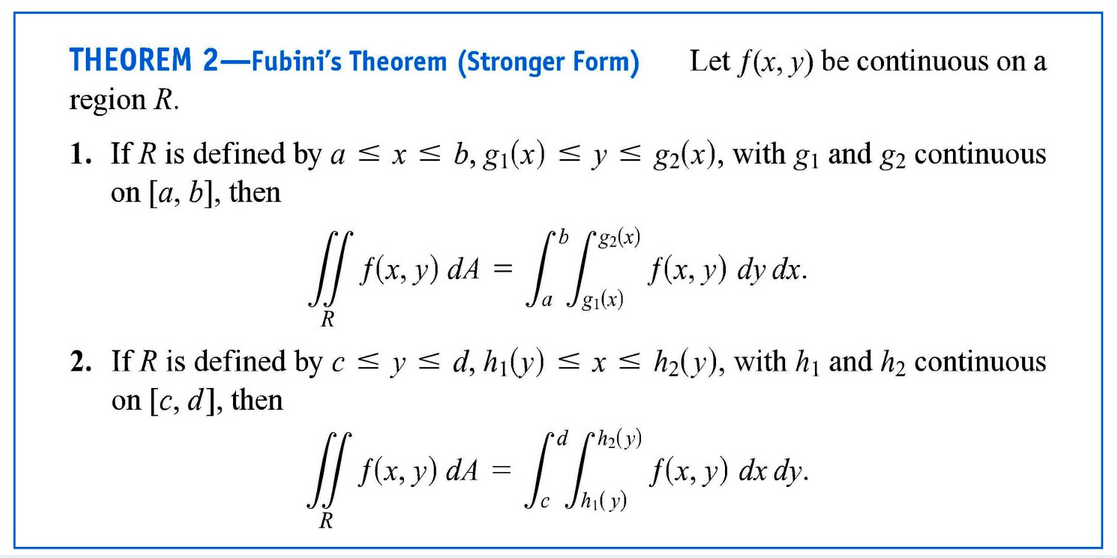
\includegraphics[width=0.8\textwidth]{Figures/pimg5.png}
    \caption{Fubini's General Theorem}
    \label{fig:pimg5-fubini-s-general-theorem}
  \end{figure}
\end{definition}


\begin{eg}[Triangular Region Bounded by \(x=0\), \(y=0\), \(x+y=1\)]
  Let \(R\) be the triangular region bounded by \(x = 0\), \(y = 0\), and \(x + y = 1\). Compute \(\iint_R (x + y)\,dA\).

  The region \(R = \{(x,y): 0 \leq x \leq 1,\; 0 \leq y \leq 1 - x\}\)

  \begin{align*}
    \iint_R (x + y)\,dA &= \int_0^1 \int_0^{1-x} (x + y)\,dy\,dx \\
                        &= \int_0^1 \left[ x y + \frac{1}{2} y^2 \right]_0^{1-x} dx \\
                        &= \int_0^1 \left[ x(1 - x) + \frac{1}{2}(1 - x)^2 \right] dx \\
                        &= \int_0^1 \left[ x - x^2 + \frac{1}{2}(1 - 2x + x^2) \right] dx \\
                        &= \int_0^1 \left[ x - x^2 + \frac{1}{2} - x + \frac{1}{2}x^2 \right] dx \\
                        &= \int_0^1 \left[ -\frac{1}{2}x^2 + \frac{1}{2} \right] dx \\
                        &= \left[ -\frac{1}{6}x^3 + \frac{1}{2}x \right]_0^1 = -\frac{1}{6} + \frac{1}{2} = \frac{1}{3}
  \end{align*}
\end{eg}
